Nur die elektromagnetische Wechselwirkung ist von Bedeutung. Folgende Reaktionen führen zu
Energieverlust von geladenen Teilchen in Materie:

\begin{itemize}
  \item Ionisation der Detektoratome
  \item Anregung der Detektoratome
  \item Bremsstrahlung (relevant für Elektronen/Positronen)
  \item \v{C}erenkov-Strahlung
  \item Übergangsstrahlung
\end{itemize}

\[-\left(\frac{dE}{dx}\right)_{\text{tot}} = -\left(\frac{dE}{dx}\right)_{\text{coll}}
-\left(\frac{dE}{dx}\right)_{\text{rad}} -\left(\frac{dE}{dx}\right)_{\text{pair}}
-\left(\frac{dE}{dx}\right)_{\text{photo}} -\left(\frac{dE}{dx}\right)_{\text{compton}}
-\left(\frac{dE}{dx}\right)_{\text{kal}}\]
 
Beispiel: Gesamte Energieverlustrate $-\frac{dE}{dx}$ für Myonen in Kupfer. Der
Großteil wird durch die Bethe-Bloch-Formel beschrieben (Herleitung erfolgt im nächsten Kapitel).
Unterschiedliche Energie der Projektile führt über unterschiedliche Wechselwirkung zum
Energieverlust.

\begin{figure}[H]
	\centering
	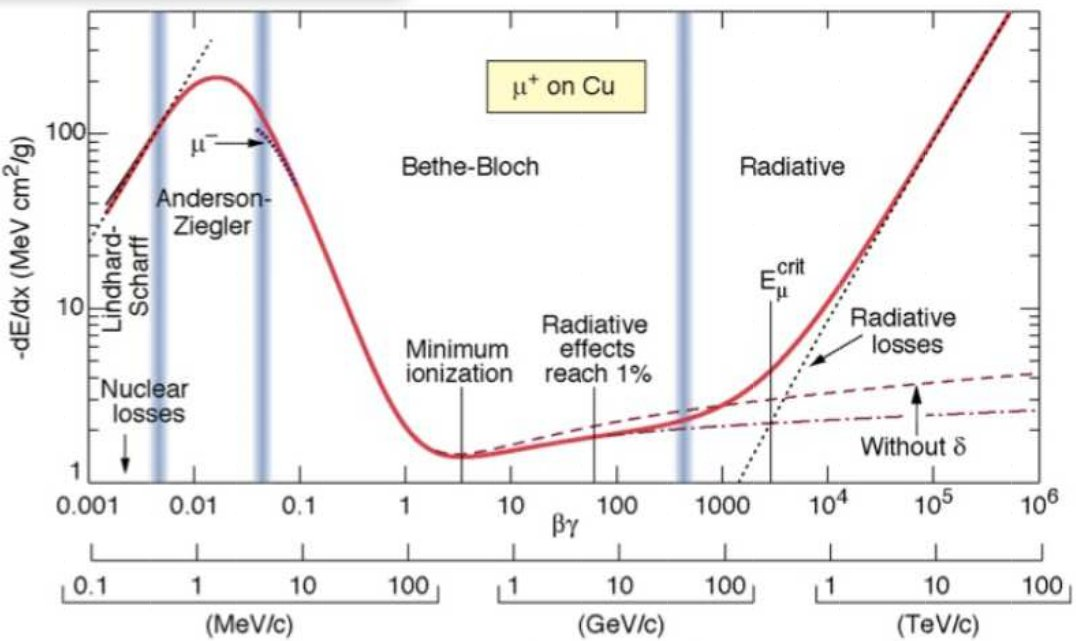
\includegraphics[width=0.5\textwidth]{bethebloch.jpg}
% 	\caption{}
% 	\label{}
\end{figure}

\begin{figure}[H]
	\centering
	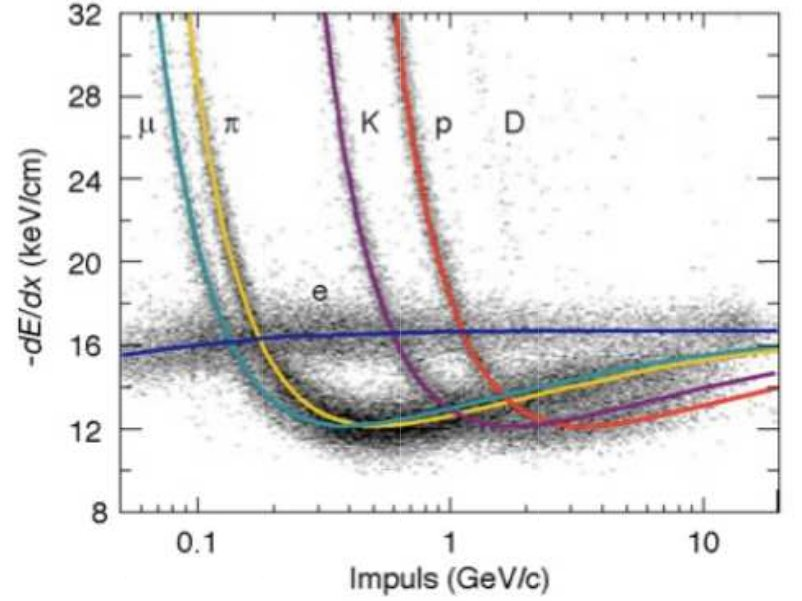
\includegraphics[width=0.5\textwidth]{bethebloch2.jpg}
	\caption{$\frac{dE}{dx}$-Kurven für verschiedene Teilchen (gemessen in der
	PEP4/9-TPC)}
	\label{}
\end{figure}
 
 Beachte: $\frac{dE}{dx}$ für "`schwere"' Teilchen (z.B. $\alpha$) wird in diesem Impulsbereich gut
 durch die Bethe-Bloch-Formel beschrieben. Der Energieverlust durch Ionisation und Anregung von
 Targetelektronen dominiert. $\frac{dE}{dx}$ für Elektronen/Positronen folgt jedoch nicht der
 Bethe-Bloch-Formel!